\documentclass[12pt,letterpaper,oneside,reqno]{amsart}
\usepackage{amsfonts}
\usepackage{amsmath}
\usepackage{amssymb}
\usepackage{amsthm}
\usepackage{float}
\usepackage[font=small,labelfont=bf]{caption}
\usepackage[left=1in,right=1in,bottom=1in,top=1in]{geometry}
\usepackage[pdfpagelabels,hyperindex,colorlinks=true,linkcolor=blue,urlcolor=magenta,citecolor=green]{hyperref}
\usepackage{graphicx}
\linespread{1.7}
\emergencystretch=1em
\usepackage{array}
\usepackage{etoolbox}
\apptocmd{\sloppy}{\hbadness 10000\relax}{}{}
\raggedbottom
\usepackage{enumitem}

\newcommand \bernoulli [2][B] {{#1}\sb{#2}}
\newcommand \coeffA [3][A] {{\mathbf{#1}} \sb{#2,#3}}
\newcommand \polynomialP [4][P]{{\mathbf{#1}}\sp{#2} \sb{#3}(#4)}

% for brack coefficient
\newcommand \brackCoefficient [3] {{#1 \brack #2}_{#3}}
\newcommand \braceCoefficient [3] {{#1 \brace #2}_{#3}}

% free foot note
\let\svthefootnote\thefootnote
\newcommand\freefootnote[1]{%
    \let\thefootnote\relax%
    \footnotetext{#1}%
    \let\thefootnote\svthefootnote%
}


\newtheorem{thm}{Theorem}[section]
\newtheorem{cor}[thm]{Corollary}
\newtheorem{lem}[thm]{Lemma}
\newtheorem{examp}[thm]{Example}
\newtheorem{conj}[thm]{Conjecture}
\newtheorem{defn}[thm]{Definition}
\newtheorem{question}[thm]{Question}
\newtheorem{assumption}[thm]{Assumption}

\title[History and overview of the polynomial \texorpdfstring{$\polynomialP{m}{b}{x}$}{P[m,b,x]}]
{History and overview of the polynomial \texorpdfstring{$\polynomialP{m}{b}{x}$}{P[m,b,x]}}
\author[Petro Kolosov]{Petro Kolosov}
\address{Software Developer, DevOps Engineer}
\email{kolosovp94@gmail.com}
\urladdr{https://kolosovpetro.github.io}
\keywords{
    Binomial theorem,
    Binomial coefficients,
    Faulhaber's formula,
    Polynomials,
    Pascal's triangle
    Finite differences,
    Interpolation,
    Polynomial identities
}
\subjclass[2010]{41-XX, 26E70, 05A30}
\date{\today}
\hypersetup{
    pdftitle={History and overview of the polynomial P(m,b,x)},
    pdfsubject={
        Polynomials,
        Finite differences,
        Interpolation,
        Approximation,
        Polynomial identities,
        Power sums,
        Binomial theorem,
        Power function,
        Binomial coefficients,
        Bernoulli numbers,
        Pascal's triangle,
        Faulhaber's formula,
        Derivatives,
        Differential calculus,
        Partial differential equations,
        OEIS,
        Bernoulli polynomials,
        Combinatorics,
        Discrete convolution,
        Dynamic systems,
        Time scales
    },
    pdfauthor={Petro Kolosov},
    pdfkeywords={
        Polynomials,
        Finite differences,
        Interpolation,
        Approximation,
        Polynomial identities,
        Power sums,
        Binomial theorem,
        Power function,
        Binomial coefficients,
        Bernoulli numbers,
        Pascal's triangle,
        Faulhaber's formula,
        Derivatives,
        Differential calculus,
        Partial differential equations,
        OEIS,
        Bernoulli polynomials,
        Combinatorics,
        Discrete convolution,
        Dynamic systems,
        Time scales
    }
}
\begin{document}
    \begin{abstract}
        The polynomial $\mathbf{P}^m_b(x)$ is a $2m+1$ degree polynomial in $(x,b) \in \mathbb{R}$
defined by a polynomial identity for odd-powers such that derived applying certain interpolation approaches.
This manuscript provides a comprehensive historical survey of the milestones and evolution of the polynomial
$\mathbf{P}^m_b(x)$, continuing with related works based on it.
%In particular, the polynomial $\mathbf{P}^m_b(x)$ establishes a relation between
%ordinary and partial derivatives of odd-powers.
%Also, it gives an opportunity to express odd-power identity in terms of multiplication of certain matrices.

%such that derived applying certain methods of interpolation, so that initially we reach the base case for $m=1$
%generalizing it up to $m\in\mathbb{N}$ afterward.
%In particular, the polynomial $\mathbf{P}^m_b(x)$ may be successfully applicable
%for polynomial interpolation and approximation approaches.
%This manuscript provides a comprehensive historical survey of the milestones and evolution of $\mathbf{P}^m_b(x)$
%as well as related works such that based onto, for instance various polynomial identities, differential equations etc.
%In addition, future research directions are proposed and discussed.

    \end{abstract}

    \maketitle

    \tableofcontents

    \freefootnote{Sources: \url{https://github.com/kolosovpetro/HistoryAndOverviewOfPolynomialP}}


    \section{History and evolution of the polynomial \texorpdfstring{$\polynomialP{m}{b}{x}$}{P[m,b,x]}}
    \label{sec:history-and-evolution-of-the-topic}
    \freefootnote{Sources: \url{https://github.com/kolosovpetro/HistoryAndOverviewOfPolynomialP}}
Back than, in 2016 being a student of faculty of mechanical engineering,
I remember myself playing with finite differences of polynomial $n^3$ over the domain of natural numbers $n\in\mathbb{N}$
having at most $0 \leq n \leq 20$ values.
Looking to the values in my finite difference tables, the first and very naive question that came to my mind was
\begin{center}
    \textit{Is it possible to re-assemble the value of
    the polynomial $n^3$ backwards having its finite differences?}
\end{center}
The answer to this question is definitely \textit{Yes}, utilizing the interpolation principles.
Interpolation is a process of finding new data points based on the range of a discrete set of known data points.
Interpolation has been well-developed in between 1674--1684
by Issac Newton's fundamental works, nowadays known as foundation of classical interpolation
theory~\cite{meijering2002chronology}.

That time, in 2016, I was a first-year mechanical engineering undergraduate,
so that due to lack of knowledge and perspective of view I started re-inventing interpolation
formula myself, fueled by purest passion and feeling of mystery.
All mathematical laws and relations exist from the very beginning, but we only find and describe them, I thought.
That mindset truly inspired me so that my own mathematical journey has been started.
Let us begin considering the table of finite differences of the polynomial $n^3$
\begin{table}[H]
    \begin{center}
        \setlength\extrarowheight{-6pt}
        \begin{tabular}{c|cccc}
            $n$ & $n^3$ & $\Delta(n^3)$ & $\Delta^2(n^3)$ & $\Delta^3(n^3)$ \\
            \hline
            0   & 0     & 1             & 6               & 6               \\
            1   & 1     & 7             & 12              & 6               \\
            2   & 8     & 19            & 18              & 6               \\
            3   & 27    & 37            & 24              & 6               \\
            4   & 64    & 61            & 30              & 6               \\
            5   & 125   & 91            & 36              &                 \\
            6   & 216   & 127           &                 &                 \\
            7   & 343   &               &                 &
        \end{tabular}
    \end{center}
    \caption{Table of finite differences of the polynomial $n^3$.} \label{tab:table}
\end{table}
First and foremost, we can observe that finite difference $\Delta(n^3)$ of the polynomial $n^3$
can be expressed via summation over $n$, e.g
\begin{align}
    \label{eq:cubes_interpolation}
    \begin{split}
        \Delta(0^3) &= 1+6 \cdot 0 \\
        \Delta(1^3) &= 1+6\cdot0+6\cdot1 \\
        \Delta(2^3) &= 1+6\cdot0+6\cdot1+6\cdot2 \\
        \Delta(3^3) &= 1+6\cdot0+6\cdot1+6\cdot2+6\cdot3 \\
        &\; \; \vdots
    \end{split}
\end{align}
Finally reaching the general one form
\begin{equation}
    \Delta(n^3) = 1+6\cdot0+6\cdot1+6\cdot2+6\cdot3+\cdots+6\cdot n = 1 + 6 \sum_{k=0}^{n} k\label{eq:general-cube-eq}
\end{equation}
The one experienced mathematician would immediately notice a spot to apply Faulhaber's formula~\cite{beardon1996sums}
to expand the term $\sum_{k=0}^{n} k$ reaching expected result that matches Binomial theorem~\cite{abramowitz1988handbook},
so that
\begin{equation*}
    \sum_{k=0}^{n} k = \frac{1}{2}(n+n^2)
\end{equation*}
Then ours relation~\eqref{eq:general-cube-eq} immediately turns into Binomial expansion
\begin{equation}
    \Delta(n^3) = (n+1)^3 - n^3 = 1 + 6 \left[ \frac{1}{2}(n+n^2) \right] = 1 + 3 n + 3 n^2 = \sum_{k=0}^{2} \binom{3}{k} n^k
    \label{eq:cubes-difference-binomial-theorem}
\end{equation}
However, as it said, I was not the experienced one mathematician back than,
so that I reviewed the relation~\eqref{eq:general-cube-eq} from a little bit different perspective.
Not following the convenient solution~\eqref{eq:cubes-difference-binomial-theorem},
I have rearranged the first order finite differences from the table~\eqref{tab:table} using~\eqref{eq:cubes_interpolation}
to get the polynomial $n^3$
\begin{align*}
    n^3 &= [1+6\cdot0]+[1+6\cdot0+6\cdot1]+[1+6\cdot0+6\cdot1+6\cdot2]+\cdots \\
    &+[1+6\cdot0+6\cdot1+6\cdot2+\cdots+6\cdot(n-1)]
\end{align*}
Then, combining above equation under the summation in terms of $(n-k)$
\begin{equation*}
    \begin{split}
        n^3 &= n + [(n-0) \cdot 6 \cdot 0] + [(n-1)\cdot6\cdot1] + [(n-2)\cdot6\cdot2] + \cdots \\
            &\cdots + [(n-k)\cdot 6 \cdot k] + \cdots + [1\cdot6\cdot(n-1)]
    \end{split}
\end{equation*}
We have successfully reached interpolation of the polynomial $n^3$
\begin{equation}
    \label{eq:cube_identity}
    n^3 = \sum_{k=1}^{n} 6k(n-k) + 1
\end{equation}
It is immediately seen that~\eqref{eq:cube_identity} holds by observing the table of $6k(n-k) + 1$ values
\begin{table}[H]
    \setlength\extrarowheight{-6pt}
    \begin{tabular}{c|cccccccc}
        $n/k$ & 0 & 1  & 2  & 3  & 4  & 5  & 6  & 7 \\
        \hline
        0     & 1 &    &    &    &    &    &    &   \\
        1     & 1 & 1  &    &    &    &    &    &   \\
        2     & 1 & 7  & 1  &    &    &    &    &   \\
        3     & 1 & 13 & 13 & 1  &    &    &    &   \\
        4     & 1 & 19 & 25 & 19 & 1  &    &    &   \\
        5     & 1 & 25 & 37 & 37 & 25 & 1  &    &   \\
        6     & 1 & 31 & 49 & 55 & 49 & 31 & 1  &   \\
        7     & 1 & 37 & 61 & 73 & 73 & 61 & 37 & 1
    \end{tabular}
    \caption{Values of $6k(n-k) + 1$.
    See the OEIS entry: \href{https://oeis.org/A287326}{\texttt{A287326}}~\cite{kolosov2017third}.
    Sequences such that row sums give the polynomials $n^{5}$ and $n^7$
    are also registered in the OEIS~\cite{kolosov2018fifth, kolosov2018seventh}.}
    \label{tab:fig_1}
\end{table}
Therefore, we have reached our base case by successfully interpolating the polynomial $n^3$.
Fairly enough that the next curiosity would be
\begin{center}
    \textit{Well, if the relation~\eqref{eq:cube_identity} true for the polynomial $n^3$,
        then is it true that~\eqref{eq:cube_identity} can be generalized for higher powers, e.g. for $n^4$ or $n^5$ either?}
\end{center}
That was my next question, however without any expectation of the form of generalized relation.
Soon enough my idea was caught by other people.
In 2018, Albert Tkaczyk has published two of his works~\cite{tkaczyk2018problem, tkaczyk2018continuation}
showing the cases for polynomials $n^5, \; n^7$ and $n^9$ obtained similarly as~\eqref{eq:cube_identity}.
In short, it appeared that relation~\eqref{eq:cube_identity} could be generalized
for any odd-power $2m+1$ solving certain system of linear equations.
It was proposed that case for $n^5$ has explicit form as
\begin{equation*}
    n^5 = \sum_{k=1}^{n} \left[ A k^2(n-k)^2 + Bk(n-k) + C \right]
\end{equation*}
where $A,B,C$ are unknown real coefficients.
Denote $A,B,C$ as $\coeffA{2}{0}, \coeffA{2}{1}, \coeffA{2}{2}$ respectively
so that we reach the form of compact double sum
\begin{equation*}
    n^5 = \sum_{k=1}^{n} \sum_{r=0}^{2} \coeffA{2}{r} k^r (n-k)^r
\end{equation*}
Now the potential form generalized of odd-power identity becomes more obvious.
To evaluate the coefficients $\coeffA{2}{0}, \coeffA{2}{1}, \coeffA{2}{2}$
we construct the system of linear equations.
In its explicit form
\begin{equation*}
    \begin{split}
        n^5 &= \sum_{r=0}^{2} \coeffA{2}{r} \sum_{k=1}^{n} k^r (n-k)^r \\
        &= \coeffA{2}{0} \sum_{k=1}^{n} k^0 (n-k)^0 + \coeffA{2}{1} \sum_{k=1}^{n} k^1 (n-k)^1 + \coeffA{2}{2} \sum_{k=1}^{n} k^2 (n-k)^2
    \end{split}
\end{equation*}
Expanding the terms $\sum_{k=1}^{n} k^r (n-k)^r$ applying the
Faulhaber's formula $\sum_{k=1}^{n}k^{p} = \frac{1}{p+1} \sum_{j=0}^{p} \binom{p+1}{j} B_{j} n^{p+1-j}$, we get the equation
\begin{equation*}
    \coeffA{m}{0} n
    + \coeffA{m}{1} \left[ \frac{1}{6} (-n + n^3) \right]
    + \coeffA{m}{2} \left[ \frac{1}{30} (-n + n^5) \right] - n^5 = 0
\end{equation*}
Multiplying by $30$ both right-hand side and left-hand side, we get
\begin{equation*}
    30 \coeffA{2}{0} n + 5 \coeffA{2}{1} (-n + n^3) + \coeffA{2}{2} (-n + n^5) - 30n^5 = 0
\end{equation*}
Expanding the brackets and rearranging the terms gives
\begin{equation*}
    30 \coeffA{2}{0} - 5 \coeffA{2}{1} n + 5 \coeffA{2}{1} n^3 - \coeffA{2}{2} n + \coeffA{2}{2} n^5 - 30n^5 = 0
\end{equation*}
Combining the common terms yields
\begin{equation*}
    n (30 \coeffA{2}{0} - 5 \coeffA{2}{1} - \coeffA{2}{2}) + 5 \coeffA{2}{1} n^3 + n^5 (\coeffA{2}{2} - 30) = 0
\end{equation*}
Therefore, the system of linear equations follows
\begin{equation*}
    \begin{cases}
        30 \coeffA{2}{0} - 5 \coeffA{2}{1} - \coeffA{2}{2} = 0 \\
        \coeffA{2}{1} = 0 \\
        \coeffA{2}{2} - 30 = 0
    \end{cases}
\end{equation*}
Solving it, we get
\begin{equation*}
    \begin{cases}
        \coeffA{2}{2} = 30 \\
        \coeffA{2}{1} = 0 \\
        \coeffA{2}{0} = 1
    \end{cases}
\end{equation*}
So that odd-power identity holds
\begin{equation*}
    n^5 = \sum_{k=1}^{n} 30k^2(n-k)^2 + 1
\end{equation*}
It is also clearly seen
why the above identity is true arranging the terms $30k^2(n-k)^2 + 1$ over $0 \leq k \leq n$ in table as
it is shown in the OEIS sequence~\cite{kolosov2018fifth}.

Therefore, the relation~\eqref{eq:cube_identity} we got previously via interpolation of the polynomial $n^3$
can be generalized for all odd-powers $2m+1$ by constructing and solving certain system of linear equations,
and its generalized form to be
\begin{equation}
    n^{2m+1} = \sum_{r=0}^{m} \coeffA{m}{r} \sum_{k=1}^{n} k^{r} (n-k)^{r}\label{eq:odd-power-identity}
\end{equation}
where $\coeffA{m}{r}$ are real coefficients.
In more details, the equation~\eqref{eq:odd-power-identity} is discussed
separately in~\cite{kolosov2022106, kolosov2023polynomial}.
However, constructing and solving systems of linear equations each time for every odd-power $2m+1$ requires huge effort,
there must be a function that generates the set of real coefficients $\coeffA{m}{r}$, I thought.
As it turned out, that assumption was correct.
So that I reached MathOverflow community in search of answers that arrived quite shortly.
In~\cite{alekseyev2018mathoverflow}, Dr. Max Alekseyev has provided a complete and comprehensive formula to calculate
coefficient $\coeffA{m}{r}$ for each natural $m\geq 0, \; 0 \leq r \leq m$.
The main idea of Alekseyev's approach was to utilize dynamic programming methods to evaluate $\coeffA{m}{r}$ recursively,
taking base case $\coeffA{m}{m}$ evaluating next $\coeffA{m}{m-1}$ via backtracking,
continuing similarly up to $\coeffA{m}{0}$.
Before we consider the derivation of the coefficients $\coeffA{m}{r}$,
a few words must be said regarding the Faulhaber's formula
\begin{equation*}
    \sum_{k=1}^{n} k^{p} = \frac{1}{p+1}\sum_{j=0}^{p} \binom{p+1}{j} \bernoulli{j} n^{p+1-j}
\end{equation*}
it is important to note that summation bound is $p$ while binomial coefficient upper bound is $p+1$.
It means that we cannot omit summation bounds letting $j$ run over infinity, unless we do some trick as
\begin{equation*}
    \begin{split}
        \sum_{k=1}^{n} k^{p}
        = \frac{1}{p+1}\sum_{j=0}^{p} \binom{p+1}{j} \bernoulli{j} n^{p+1-j}
        &= \left[ \frac{1}{p+1}\sum_{j=0}^{p+1} \binom{p+1}{j} \bernoulli{j} n^{p+1-j} \right] - \bernoulli{p+1} \\
        &= \left[ \frac{1}{p+1}\sum_{j} \binom{p+1}{j} \bernoulli{j} n^{p+1-j} \right] - \bernoulli{p+1}
    \end{split}
\end{equation*}
So that now we consider the derivation of coefficients $\coeffA{m}{r}$.
Using the Faulhaber's formula
$\sum_{k=1}^{n} k^{p} = \left[ \frac{1}{p+1}\sum_{j} \binom{p+1}{j} \bernoulli{j} n^{p+1-j} \right] - \bernoulli{p+1}$
we get
\begin{equation*}
    \begin{split}
        &\sum_{k=1}^{n} k^{r} (n-k)^{r}
        = \sum_{t=0}^{r} (-1)^t \binom{r}{t} n^{r-t} \sum_{k=1}^{n} k^{t+r} \\
        &= \sum_{t=0}^{r} (-1)^t \binom{r}{t} n^{r-t} \left[ \frac{1}{t+r+1} \sum_{j} \binom{t+r+1}{j} \bernoulli{j} n^{t+r+1-j} - \bernoulli{t+r+1} \right] \\
        &= \sum_{t=0}^{r} \binom{r}{t} \left[ \frac{(-1)^t}{t+r+1} \sum_{j} \binom{t+r+1}{j} \bernoulli{j} n^{2r+1-j} - \bernoulli{t+r+1} n^{r-t} \right] \\
        &= \sum_{t=0}^{r} \binom{r}{t} \frac{(-1)^t}{t+r+1} \sum_{j} \binom{t+r+1}{j} \bernoulli{j} n^{2r+1-j} - \sum_{t=0}^{r} \binom{r}{t} \frac{(-1)^t}{t+r+1} \bernoulli{t+r+1} n^{r-t} \\
        &= \sum_{j} \sum_{t} \binom{r}{t} \frac{(-1)^t}{t+r+1} \binom{t+r+1}{j} \bernoulli{j} n^{2r+1-j} - \sum_{t=0}^{r} \binom{r}{t} \frac{(-1)^t}{t+r+1} \bernoulli{t+r+1} n^{r-t} \\
        &= \sum_{j} \bernoulli{j} n^{2r+1-j} \sum_{t} \binom{r}{t} \frac{(-1)^t}{t+r+1} \binom{t+r+1}{j} - \sum_{t=0}^{r} \binom{r}{t} \frac{(-1)^t}{t+r+1} \bernoulli{t+r+1} n^{r-t}
    \end{split}
\end{equation*}
Now, we notice that
\begin{equation}
    \sum_{t} \binom{r}{t} \frac{(-1)^t}{r+t+1} \binom{r+t+1}{j}
    =\begin{cases}
         \frac{1}{(2r+1) \binom{2r}r}, & \text{if } j=0;\\
         \frac{(-1)^r}{j} \binom{r}{2r-j+1}, & \text{if } j>0.
    \end{cases}\label{eq:combinatorial-identity}
\end{equation}
An elegant proof of the above binomial identity is provided at~\cite{scheuer2023mathstackexchange}.
In particular, the equation~\eqref{eq:combinatorial-identity} is zero for $0< t \leq j$.
So that taking $j=0$ we have
\begin{equation*}
    \begin{split}
        \sum_{k=1}^{n} k^{r} (n-k)^{r}
        &= \frac{1}{(2r+1) \binom{2r}r} n^{2r+1} + \left[ \sum_{j \geq 1} \bernoulli{j} n^{2r+1-j} \sum_{t} \binom{r}{t} \frac{(-1)^t}{t+r+1} \binom{t+r+1}{j} \right] \\
        &- \left[ \sum_{t=0}^{r} \binom{r}{t} \frac{(-1)^t}{t+r+1} \bernoulli{t+r+1} n^{r-t} \right]
    \end{split}
\end{equation*}
Now let's simplify the double summation applying the identity~\eqref{eq:combinatorial-identity}
\begin{equation*}
    \begin{split}
        \sum_{k=1}^{n} k^{r} (n-k)^{r}
        &= \frac{1}{(2r+1) \binom{2r}r} n^{2r+1}
        + \underbrace{\left[ \sum_{j \geq 1} \frac{(-1)^r}{j} \binom{r}{2r-j+1} \bernoulli{j} n^{2r+1-j} \right]}_{(\star)} \\
        &- \underbrace{\left[ \sum_{t=0}^{r} \binom{r}{t} \frac{(-1)^t}{t+r+1} \bernoulli{t+r+1} n^{r-t} \right]}_{(\diamond)}
    \end{split}
\end{equation*}
Hence, introducing $\ell=2r-j+1$ to $(\star)$ and $\ell=r-t$ to $(\diamond)$ we collapse the common terms of the above
equation so that we get
\begin{equation*}
    \begin{split}
        \sum_{k=1}^{n} k^{r} (n-k)^{r}
        &= \frac{1}{(2r+1) \binom{2r}r} n^{2r+1}
        + \left[ \sum_{\ell} \frac{(-1)^r}{2r+1-\ell} \binom{r}{\ell} \bernoulli{2r+1-\ell} n^{\ell} \right] \\
        &- \left[ \sum_{\ell} \binom{r}{\ell} \frac{(-1)^{r-\ell}}{2r+1-\ell} \bernoulli{2r+1-\ell} n^{\ell} \right]\\
        &= \frac{1}{(2r+1) \binom{2r}r} n^{2r+1} + 2 \sum_{\mathrm{odd \; \ell}} \frac{(-1)^r}{2r+1-\ell} \binom{r}{\ell} \bernoulli{2r+1-\ell} n^{\ell}
    \end{split}
\end{equation*}
Using the definition of $\coeffA{m}{r}$, we obtain the following identity for polynomials in $n$
\begin{equation*}
    \sum_{r} \coeffA{m}{r} \frac{1}{(2r+1) \binom{2r}r} n^{2r+1}
    + 2 \sum_{r} \coeffA{m}{r} \sum_{\mathrm{odd \; \ell}} \frac{(-1)^r}{2r+1-\ell} \binom{r}{\ell} \bernoulli{2r+1-\ell} n^{\ell}
    \equiv n^{2m+1}
\end{equation*}
Replacing odd $\ell$ by $d$ we get
\begin{equation}
    \begin{split}
        &\sum_{r} \coeffA{m}{r} \frac{1}{(2r+1) \binom{2r}r} n^{2r+1}
        + 2 \sum_{r} \coeffA{m}{r} \sum_{d} \frac{(-1)^r}{2r-2d} \binom{r}{2d+1} \bernoulli{2r-2d} n^{2d+1}
        \equiv n^{2m+1} \\
        &\sum_{r} \coeffA{m}{r} \left[ \frac{1}{(2r+1) \binom{2r}r} n^{2r+1} \right]
        + 2 \sum_{r} \coeffA{m}{r} \left[ \sum_{d} \frac{(-1)^r}{2r-2d} \binom{r}{2d+1} \bernoulli{2r-2d} n^{2d+1} \right]
        - n^{2m+1} = 0
%        \\
%        &\sum_{r=0}^{m} \coeffA{m}{r} \left[ \frac{1}{(2r+1) \binom{2r}r} n^{2r+1} \right]
%        + 2 \sum_{r=0}^{m} \coeffA{m}{r} \left[ \sum_{d=0}^{(r-1)/2} \frac{(-1)^r}{2r-2d} \binom{r}{2d+1} \bernoulli{2r-2d} n^{2d+1} \right]
%        - n^{2m+1} = 0
    \end{split}\label{eq:equation7}
\end{equation}
Taking the coefficient of $n^{2m+1}$ in~\eqref{eq:equation7}, we get
\begin{equation*}
    \coeffA{m}{m} = (2m+1)\binom{2m}{m}
\end{equation*}
and taking the coefficient of $n^{2d+1}$ for an integer $d$ in the range $m/2 \leq d < m$, we get
\begin{equation*}
    \coeffA{m}{d} = 0
\end{equation*}
Taking the coefficient of $n^{2d+1}$ for $d$ in the range $m/4 \leq d < m/2$ we get
\begin{equation*}
    \coeffA{m}{d} \frac{1}{(2d+1) \binom{2d}{d}}
    +2 (2m+1) \binom{2m}{m}\binom{m}{2d+1} \frac{(-1)^m}{2m-2d} \bernoulli{2m-2d} = 0
\end{equation*}
i.e
\begin{equation*}
    \coeffA{m}{d} = (-1)^{m-1} \frac{(2m+1)!}{d!d!m!(m-2d-1)!} \frac{1}{m-d} \bernoulli{2m-2d}
\end{equation*}
Continue similarly we can express $\coeffA{m}{r}$ for each integer $r$ in range $m/2^{s+1}\leq r < m/2^s$
(iterating consecutively $s=1,2,\ldots$) via previously determined values of $\coeffA{m}{d}$ as follows
\begin{equation*}
    \coeffA{m}{r} =
    (2r+1) \binom{2r}{r} \sum_{d \geq 2r+1}^{m} \coeffA{m}{d} \binom{d}{2r+1} \frac{(-1)^{d-1}}{d-r}
    \bernoulli{2d-2r}
\end{equation*}
Finally, the coefficient $\coeffA{m}{r}$ is defined recursively as
\begin{equation}
    \label{eq:definition_coefficient_a}
    \coeffA{m}{r} \colonequals
    \begin{cases}
    (2r+1)
        \binom{2r}{r}, & \text{if } r=m; \\
        (2r+1) \binom{2r}{r} \sum_{d \geq 2r+1}^{m} \coeffA{m}{d} \binom{d}{2r+1} \frac{(-1)^{d-1}}{d-r}
        \bernoulli{2d-2r}, & \text{if } 0 \leq r<m; \\
        0, & \text{if } r<0 \text{ or } r>m,
    \end{cases}
\end{equation}
where $\bernoulli{t}$ are Bernoulli numbers~\cite{bateman1953higher}.
It is assumed that $\bernoulli{1}=\frac{1}{2}$.
For example,
\begin{table}[H]
    \begin{center}
        \setlength\extrarowheight{-6pt}
        \begin{tabular}{c|cccccccc}
            $m/r$ & 0 & 1       & 2      & 3      & 4   & 5    & 6     & 7 \\ [3px]
            \hline
            0     & 1 &         &        &        &     &      &       &       \\
            1     & 1 & 6       &        &        &     &      &       &       \\
            2     & 1 & 0       & 30     &        &     &      &       &       \\
            3     & 1 & -14     & 0      & 140    &     &      &       &       \\
            4     & 1 & -120    & 0      & 0      & 630 &      &       &       \\
            5     & 1 & -1386   & 660    & 0      & 0   & 2772 &       &       \\
            6     & 1 & -21840  & 18018  & 0      & 0   & 0    & 12012 &       \\
            7     & 1 & -450054 & 491400 & -60060 & 0   & 0    & 0     & 51480
        \end{tabular}
    \end{center}
    \caption{Coefficients $\coeffA{m}{r}$.}
    \label{tab:table_of_coefficients_a}
\end{table}
The nominators and denominators of the coefficients $\coeffA{m}{r}$ are also registered as sequences in
the OEIS~\cite{kolosov2018numerator,kolosov2018denominator}, respectively.
It is as well interesting to notice that row sums of the $\coeffA{m}{r}$ give powers of $2$
\begin{equation*}
    \sum_{r=0}^{m} \coeffA{m}{r} = 2^{2m+1} - 1
\end{equation*}
Therefore, we have successfully shown and generalized previously obtained equation~\eqref{eq:cube_identity}
\begin{thm}
    For every $n\geq 1, \; n,m\in\mathbb{N}$ there are $\coeffA{m}{0}, \coeffA{m}{1},\dots,\coeffA{m}{m}$,
    such that
    \begin{equation*}
        n^{2m+1} = \sum_{k=1}^{n}\sum_{r=0}^{m} \coeffA{m}{r} k^r (n-k)^r
        \label{eq:odd-power-theorem}
    \end{equation*}
    where $\coeffA{m}{r}$ is a real coefficient defined recursively by~\eqref{eq:definition_coefficient_a}.
\end{thm}
Theorem~\eqref{eq:odd-power-theorem} can be considered as succeeded interpolation of the polynomial $x^{2m+1}$
over the domains $n\in\mathbb{R}, \; m\in\mathbb{N}$.

Finally, we got our road to the main definition of polynomial $\polynomialP{m}{b}{x}$
as it is closely related to the equation~\eqref{eq:odd-power-theorem}.
So let's define it without further hesitation
\begin{defn} (Polynomial $\polynomialP{m}{b}{x} $of degree $2m+1$.)
    \begin{equation}
        \polynomialP{m}{b}{x} = \sum_{k=0}^{b-1} \sum_{r=0}^{m} \coeffA{m}{r} k^r(x-k)^r
        \label{eq:definition_polynomial_p}
    \end{equation}
\end{defn}
where $\coeffA{m}{r}$ are real coefficients~\eqref{eq:definition_coefficient_a}, $m\in\mathbb{N}$ and $(x, b)\in \mathbb{R}$.
A comprehensive discussion on the polynomial $\polynomialP{m}{b}{x}$ as well as its properties can be found at~\cite{kolosov2016link}.
%For example, the polynomials $\polynomialP{m}{b}{x}$ for $0\leq m\leq 3$ are
%\begin{equation*}
%    \begin{split}
%        \polynomialP{0}{b}{x}
%        &=b \\
%        \polynomialP{1}{b}{x}
%        &=3 b^2 - 2 b^3 - 3 b x + 3 b^2 x \\
%        \polynomialP{2}{b}{x}
%        &=10 b^3 - 15 b^4 + 6 b^5- 15 b^2 x + 30 b^3 x - 15 b^4 x + 5 b x^2 - 15 b^2 x^2 + 10 b^3 x^2 \\
%        \polynomialP{3}{b}{x}
%        &=-7 b^2 + 28 b^3 - 70 b^5 + 70 b^6 - 20 b^7 + 7 b x - 42 b^2 x + 175 b^4 x - 210 b^5 x + 70 b^6 x \\
%        &+ 14 b x^2 - 140 b^3 x^2 + 210 b^4 x^2 - 84 b^5 x^2 + 35 b^2 x^3 - 70 b^3 x^3 + 35 b^4 x^3
%    \end{split}
%\end{equation*}
In 2023, Albert Tkaczyk yet again extended the theorem~\eqref{eq:odd-power-theorem} to the so-called three dimension case
so that it gives polynomials of the form $n^{3l+2}$ at~\cite{albert_tkaczyk_2023_8371454}.



    \section{Related works}\label{sec:related-works}
    We show related works in format of a directed graph, where node represents
a work and edge represents a citation between two works.
For example, the node 12 (current manuscript) cites the manuscripts 7 and 8.
Nodes of the related work graph in BFS order are
\begin{itemize}
    \item {\Large \textcircled{\normalsize 12}} is this manuscript
    \item {\Large \textcircled{\normalsize 7}} is \textit{A study on partial dynamic equation on time scales involving derivatives
    of polynomials}~\cite{study_on_partial_dynamic_eq_on_time_scales_with_poly_derivatives}
    \item {\Large \textcircled{\normalsize 8}} is \textit{106.37 An unusual identity for odd-powers}~\cite{unusual_identity_for_odd_powers}
    \item {\Large \textcircled{\normalsize 9}} is \textit{Another approach to get derivative of odd-power}~\cite{another_approach_to_get_derivative_of_odd_power}
    \item {\Large \textcircled{\normalsize B}} is \textit{A two-sided Faulhaber-like formula involving Bernoulli polynomials}~\cite{barbero2020two}
    \item {\Large \textcircled{\normalsize 10}} is \textit{Polynomial identity involving Binomial Theorem and Faulhaber's formula}~\cite{polynomial_identity_with_binomial_theorem_and_faulhabers_formula}
    \item {\Large \textcircled{\normalsize 11}} is \textit{Finding the derivative of polynomials via double limit}~\cite{derivative_of_polynomials_via_double_limit}
    \item {\Large \textcircled{\normalsize 6}} is \textit{On the link between binomial theorem and discrete convolution}~\cite{on_the_link_between_binomial_theorem_and_discrete_convolution}
\end{itemize}
\begin{figure}[H]
    \centering
    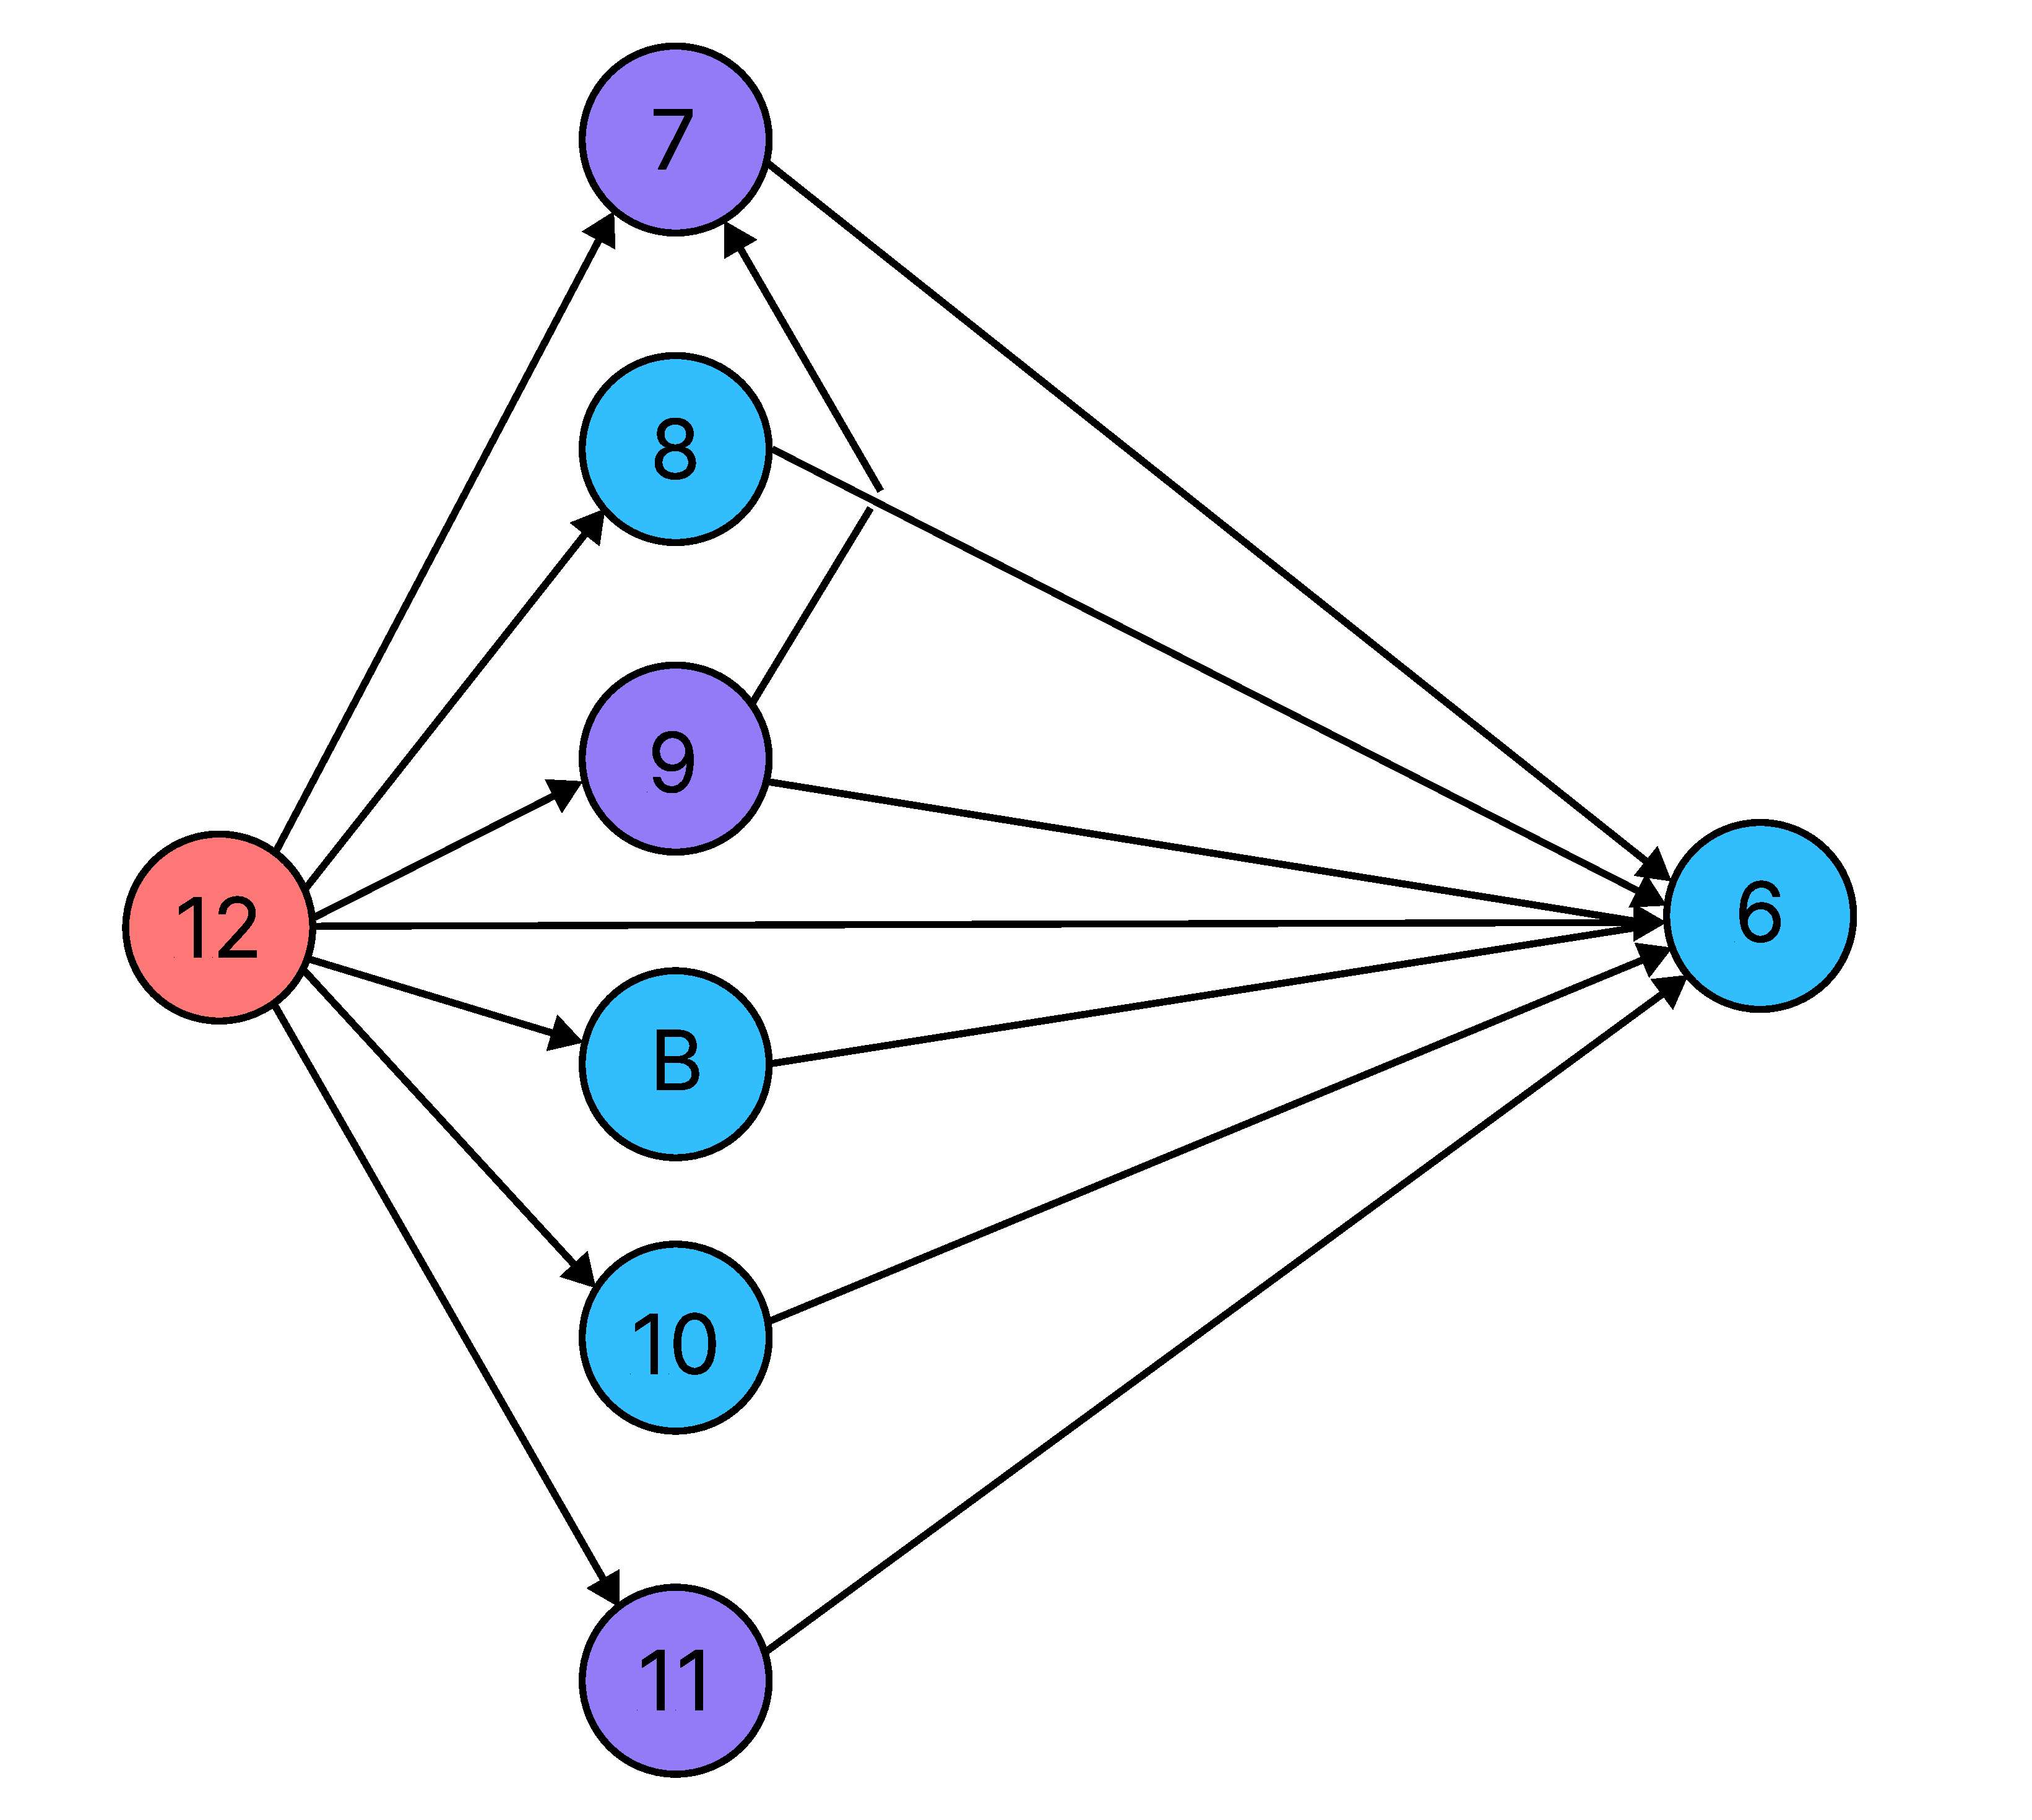
\includegraphics[width=1\textwidth]{images/realated_works_graph}
    ~\caption{Related works graph.}\label{fig:related-works-graph}
\end{figure}
\begin{itemize}
    \item {\Large \textcircled{\normalsize 12}} This manuscript
    \item {\Large \textcircled{\normalsize 6}}
    In \textit{On the link between binomial theorem and discrete convolution}~\cite{on_the_link_between_binomial_theorem_and_discrete_convolution}:
    Let $\mathbf{P}^{m}_{b}(x)$ be a $2m+1$-degree polynomial in $x$ and $b \in \mathbb{R}$
    \[
        \mathbf{P}^{m}_{b}(x) = \sum_{k=0}^{b-1} \sum_{r=0}^{m} \mathbf{A}_{m,r} k^r (x-k)^r
    \]
    where $\mathbf{A}_{m,r}$ are real coefficients.
    In this manuscript, we introduce the polynomial $\mathbf{P}^{m}_{b}(x)$ and study its properties,
    establishing a polynomial identity for odd-powers in terms of this polynomial.
    Based on mentioned polynomial identity for odd-powers,
    we explore the connection between the Binomial theorem and discrete convolution of odd-powers,
    further extending this relation to the multinomial case.
    All findings are verified using Mathematica programs.
    \item {\Large \textcircled{\normalsize 7}}
    In \textit{A study on partial dynamic equation on time scales involving derivatives
    of polynomials}~\cite{study_on_partial_dynamic_eq_on_time_scales_with_poly_derivatives}:
    Extends the main results of {\Large \textcircled{\normalsize 6}} deriving and discussing
    an identity that connects the timescale derivative of odd-powered polynomial
    with partial derivatives of polynomial $\polynomialP{m}{b}{x}$ evaluated in particular points.
    For every $t\in\mathbb{T}_1$ and $(x,b) \in \Lambda^2$
    \[
        \frac{\Delta x^{2m+1}}{\Delta x}(t) =
        \frac{\partial P(m,b,x)}{\Delta x} (m, \sigma(t), t) +
        \frac{\partial P(m,b,x)}{\Delta b} (m, t, t)
    \]
    such that $\sigma(t) > t$ is forward jump operator.
    In addition, we discuss various derivative operators in the context of the partial cases of above equation,
    We show finite difference, classical derivative, $q-$derivative, $q-$power derivative on behalf of it.
    \item {\Large \textcircled{\normalsize 8}}
    In \textit{106.37 An unusual identity for odd-powers}~\cite{unusual_identity_for_odd_powers}:
    Explores and proves the partial case of {\Large \textcircled{\normalsize 6}}
    that is the polynomial identity for odd-powers
    \[
        n^{2m+1} = \sum_{k=1}^{n} \sum_{r=0}^{m} \mathbf{A}_{m,r} k^r (n-k)^r
    \]
    \item {\Large \textcircled{\normalsize 9}}
    In \textit{Another approach to get derivative of odd-power}~\cite{another_approach_to_get_derivative_of_odd_power}:
    Extends the results of {\Large \textcircled{\normalsize 6}} by providing a relation in terms of partial differential equations such that
    ordinary derivative of odd-power $2m+1$ can be reached in terms of partial derivative of the polynomial $\polynomialP{m}{b}{x}$.
    Let be a fixed point $v\in \mathbb{N}$, then ordinary derivative $\frac{d}{dx} g_v (u)$ of the odd-power function $g_v(x) = x^{2v + 1}$
    evaluate in point $u\in\mathbb{R}$ equals to partial derivative $(f_{v})^{'}_{x} (u, u)$ evaluate in point $(u, u)$ plus
    partial derivative $(f_{v})^{'}_{z} (u, u)$ evaluate in point $(u, u)$
    \begin{equation}
        \frac{d}{dx} g_v (u) = (f_{v})^{'}_{x} (u, u) + (f_{v})^{'}_{z} (u, u)
        \label{eq:odd-exponential-identity}
    \end{equation}
    where $f_{y} (x, z) = \sum_{k=1}^{z} \sum_{r=0}^{y} \coeffA{y}{r} k^r (x-k)^r = \polynomialP{y}{z}{x}$.
    \item {\Large \textcircled{\normalsize B}}
    In \textit{A two-sided Faulhaber-like formula involving Bernoulli polynomials}~\cite{barbero2020two}:
    Based on equation~\eqref{eq:equation7}, the authors give a new identity involving
    Bernoulli polynomials and combinatorial numbers that provides,
    in particular, the Faulhaber-like formula for sums of the form $1^m(n-1)^m + 2^m (n -2)^m + \cdots + (n - 1)^m 1^m$
    for positive integers $m$ and $n$.
    \item {\Large \textcircled{\normalsize 10}}
    In \textit{Polynomial identity involving Binomial Theorem and Faulhaber's formula}~\cite{polynomial_identity_with_binomial_theorem_and_faulhabers_formula}:
    proves that
    for every $n\geq 1, \; n,m\in\mathbb{N}$
    there are coefficients $\mathbf{A}_{m,0}, \mathbf{A}_{m,1}, \ldots, \mathbf{A}_{m,m}$ such that
    the polynomial identity holds
    \[
        n^{2m+1} = \sum_{k=1}^{n} \mathbf{A}_{m,0} k^0 (n-k)^0 + \mathbf{A}_{m,1}(n-k)^1
        + \cdots + \mathbf{A}_{m,m} k^m (n-k)^m
    \]
    which is a direct consequence of the definition of $\polynomialP{m}{b}{x}$ given in {\Large \textcircled{\normalsize 6}},
    reached by utilizing Binomial theorem and Faulhaber's formula.
    \item {\Large \textcircled{\normalsize 11}}
    In \textit{Finding the derivative of polynomials via double limit}~\cite{derivative_of_polynomials_via_double_limit}:
    By applying the results of {\Large \textcircled{\normalsize 6}} provides
    another perspective of ordinary derivatives of polynomials allowing expressing
    them via a double limit, because
    \begin{align*}
        \lim_{h \to 0} \polynomialP{m}{x+h}{x} = x^{2m+1}
    \end{align*}
    \item Three sequences were contributed to the
    OEIS~\cite{oeis_coefficients_u_m_l_k_defined_by_polynomial_identity_1, oeis_coefficients_u_m_l_k_defined_by_polynomial_identity_2, oeis_coefficients_u_m_l_k_defined_by_polynomial_identity_3}
    showing the coefficients of the polynomial $\polynomialP{m}{b}{x}$ having fixed points $m,b$ while $x\in\mathbb{R}$.
    \item OEIS sequences such that row sums give odd-powers~\cite{oeis_numerical_triangle_row_sums_give_cubes, oeis_numerical_triangle_row_sums_give_fifth_powers, oeis_numerical_triangle_row_sums_give_seventh_powers}.
    \item OEIS sequences related to the coefficients $\coeffA{m}{r}$~\cite{oeis_numerators_of_the_coefficient_a_m_r, oeis_denominators_of_the_coefficient_a_m_r}.
\end{itemize}
The node indexes in the related works graph are not random, persisting the same values as
these works have on my personal website
\begin{center}
    \href{https://kolosovpetro.github.io/math/}{\texttt{kolosovpetro.github.io/math}}
\end{center}



    \section{Future research and activities}\label{sec:future-research}
    \begin{itemize}
    \item Differential equation~\eqref{eq:odd-exponential-identity} can be expressed in terms of backward
    and central differentials, as well as its dynamic equation analogs~\cite{kolosov2016study}
    \item Definition~\eqref{eq:definition_polynomial_p} is closely related to discrete convolution, probably
    some new identities in term of discrete convolution may be found
    \item All kind of derivatives (forward, backward, central), including time scale ones can be expressed
    as double limit similarly to~\cite{kolosov_2024_10575485}
    \item Equation~\eqref{eq:definition_polynomial_p} approximates odd-power $2m+1$ in some neighborhood of fixed point
    $a$ as it shown on graphs
    \begin{figure}[H]
        \centering
        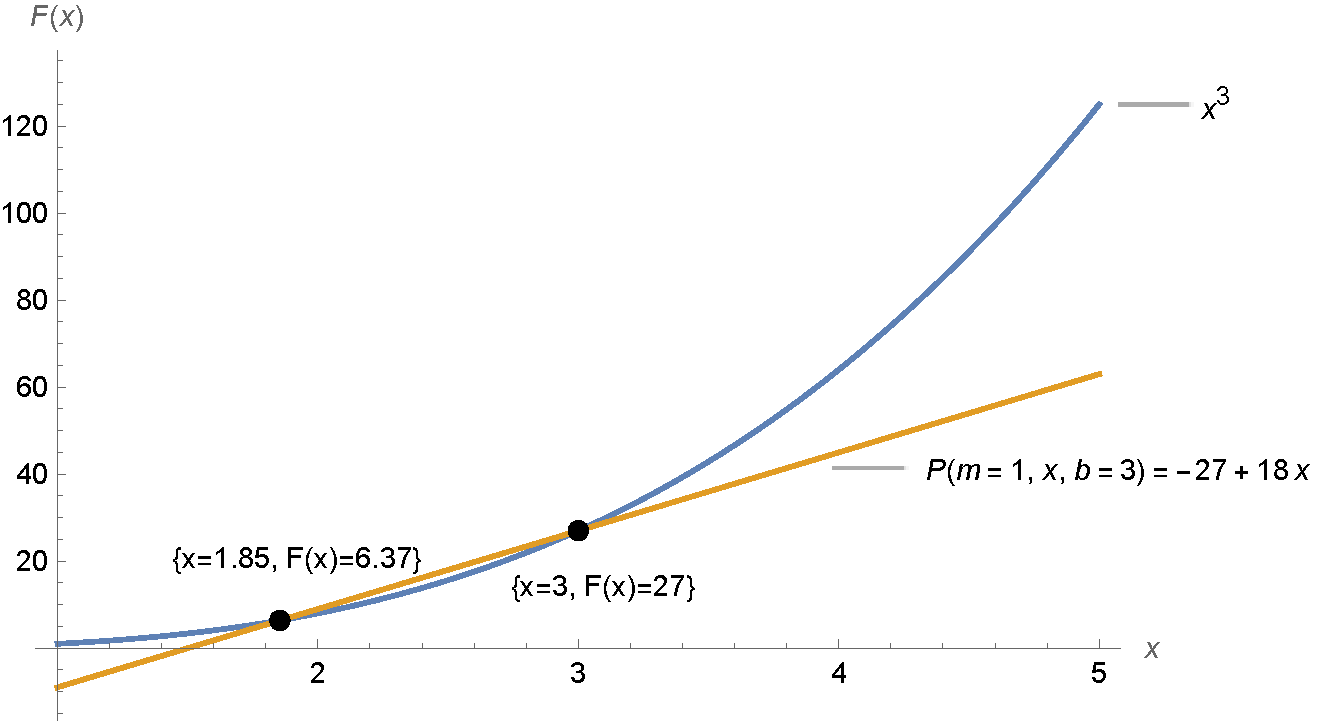
\includegraphics[width=0.6\textwidth]{images/n^3_approximation_m1_b3}
        ~\caption{Approximation of $x^3$.}\label{fig:approximation-n3}
    \end{figure}
    \begin{figure}[H]
        \centering
        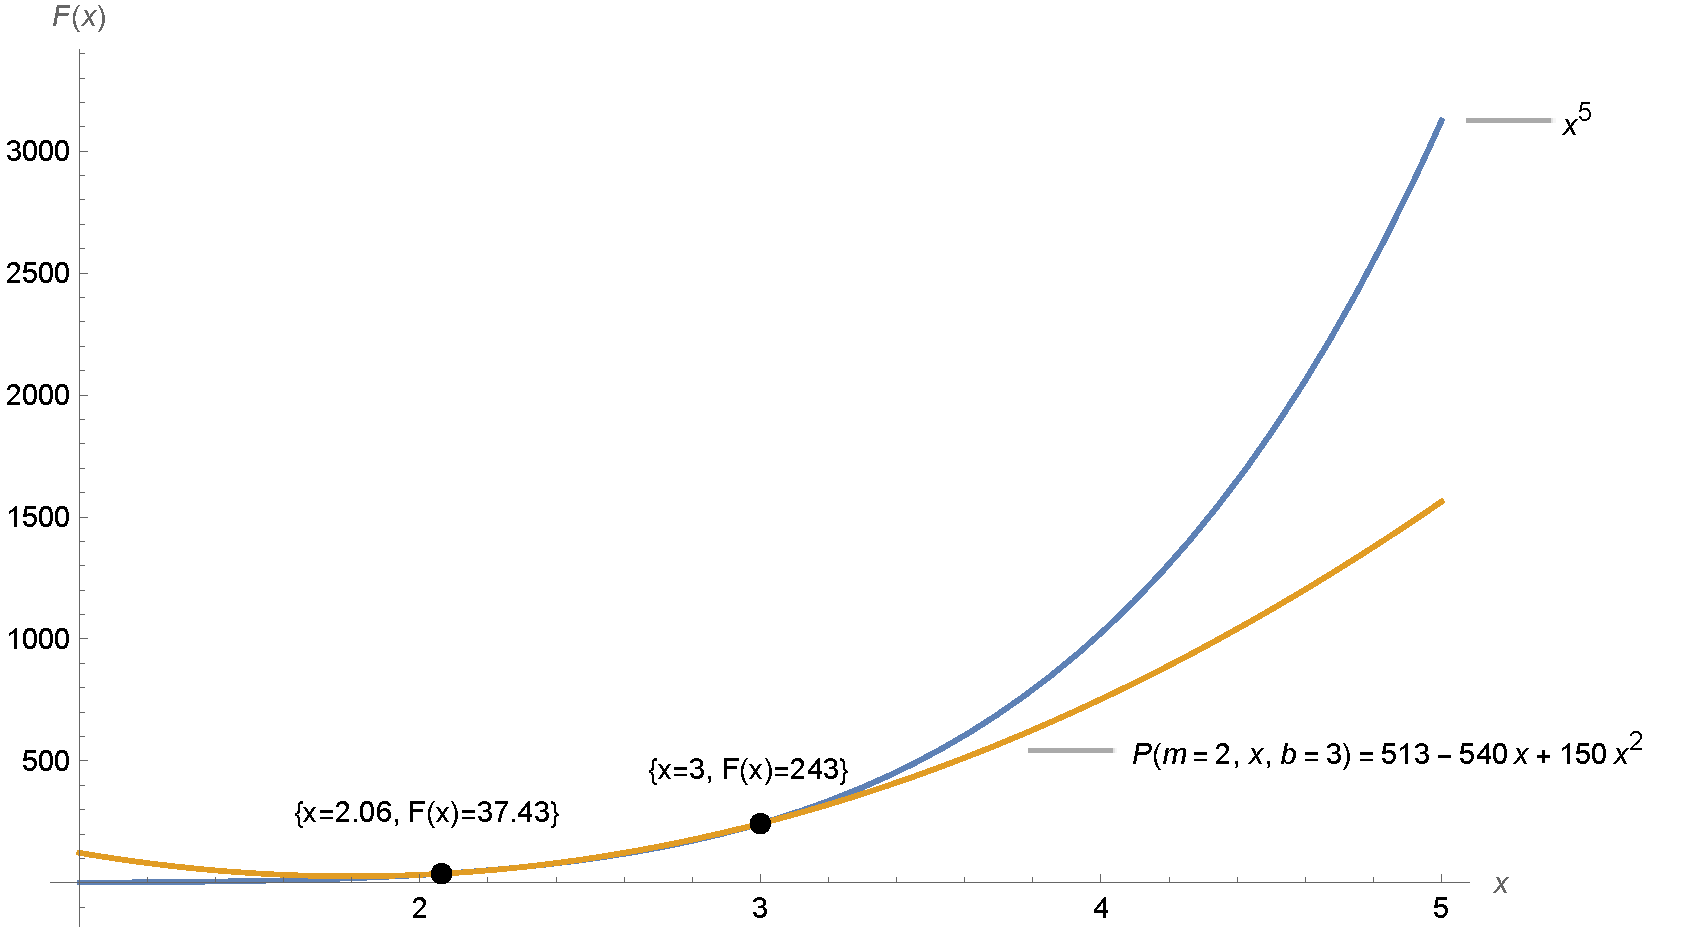
\includegraphics[width=0.6\textwidth]{images/n^5_approximation_m2_b3}
        ~\caption{Approximation of $x^5$.}\label{fig:approximation-n5}
    \end{figure}
    \item Improvements and suggestions to current manuscript via open-source activities at
    \url{https://github.com/kolosovpetro/HistoryAndOverviewOfPolynomialP}
\end{itemize}



    \section{Conclusions}\label{sec:conclusions}
    In this manuscript we have successfully provided a comprehensive historical survey
of the milestones and evolution of the polynomial $\polynomialP{m}{b}{x}$
as well as related works such that based onto, for instance various polynomial identities, differential equations etc.
In addition, future research directions are proposed and discussed.


    \bibliographystyle{unsrt}
    \bibliography{HistoryAndOverviewOfPolynomialP}
    \noindent \textbf{Version:} \texttt{Local-0.1.0}


    \section{Addendum 1: Examples of the polynomial \texorpdfstring{$\polynomialP{m}{b}{x}$}{P[m,b,x]}}
    \label{sec:addendum-1}
    \begin{equation*}
    \begin{split}
        \polynomialP{0}{b}{x}
        &=b \\
        \polynomialP{1}{b}{x}
        &=3 b^2 - 2 b^3 - 3 b x + 3 b^2 x \\
        \polynomialP{2}{b}{x}
        &=10 b^3 - 15 b^4 + 6 b^5- 15 b^2 x + 30 b^3 x - 15 b^4 x + 5 b x^2 - 15 b^2 x^2 + 10 b^3 x^2 \\
        \polynomialP{3}{b}{x}
        &=-7 b^2 + 28 b^3 - 70 b^5 + 70 b^6 - 20 b^7 + 7 b x - 42 b^2 x + 175 b^4 x - 210 b^5 x + 70 b^6 x \\
        &+ 14 b x^2 - 140 b^3 x^2 + 210 b^4 x^2 - 84 b^5 x^2 + 35 b^2 x^3 - 70 b^3 x^3 + 35 b^4 x^3 \\
        \polynomialP{4}{b}{x}
        &= -60 b^2 + 180 b^3 - 294 b^5 + 420 b^7 - 315 b^8 + 70 b^9 + 60 b x - 270 b^2 x + 735 b^4 x - 1470 b^6 x \\
        &+ 1260 b^7 x - 315 b^8 x + 90 b x^2 - 630 b^3 x^2 + 1890 b^5 x^2 - 1890 b^6 x^2 + 540 b^7 x^2 + 210 b^2 x^3 \\
        &- 1050 b^4 x^3 + 1260 b^5 x^3 - 420 b^6 x^3 - 21 b x^4 + 210 b^3 x^4 - 315 b^4 x^4 + 126 b^5 x^4\\
        \polynomialP{5}{b}{x}
        &= -693 b^2 + 2068 b^3 - 330 b^4 - 2640 b^5 + 2772 b^7 - 2310 b^9 + 1386 b^{10} - 252 b^{11} + 693 b x \\
        &- 3102 b^2 x + 660 b^3 x + 6600 b^4 x - 9702 b^6 x + 10395 b^8 x - 6930 b^9 x + 1386 b^{10} x + 1034 b x^2 \\
        &- 330 b^2 x^2 - 5940 b^3 x^2 + 12936 b^5 x^2 - 18480 b^7 x^2 + 13860 b^8 x^2 - 3080 b^9 x^2 + 2310 b^2 x^3 \\
        &- 8085 b^4 x^3 + 16170 b^6 x^3 - 13860 b^7 x^3 + 3465 b^8 x^3 - 330 b x^4 + 2310 b^3 x^4 - 6930 b^5 x^4 \\
        &+ 6930 b^6 x^4 - 1980 b^7 x^4 - 231 b^2 x^5 + 1155 b^4 x^5 - 1386 b^5 x^5 + 462 b^6 x^5 \\
        \polynomialP{6}{b}{x}
        &= -10920 b^2 + 33306 b^3 - 9009 b^4 - 36036 b^5 + 37752 b^7 - 22022 b^9 + 12012 b^{11} - 6006 b^{12} + 924 b^{13} \\
        &+ 10920 b x - 49959 b^2 x + 18018 b^3 x + 90090 b^4 x - 132132 b^6 x + 99099 b^8 x - 66066 b^{10} x + 36036 b^{11} x \\
        &- 6006 b^{12} x + 16653 b x^2 - 9009 b^2 x^2 - 84084 b^3 x^2 + 180180 b^5 x^2 - 180180 b^7 x^2 + 150150 b^9 x^2 \\
        &- 90090 b^{10} x^2 + 16380 b^{11} x^2 + 36036 b^2 x^3 - 120120 b^4 x^3 + 168168 b^6 x^3 - 180180 b^8 x^3 \\
        &+ 120120 b^9 x^3 - 24024 b^{10} x^3 - 6006 b x^4 + 40040 b^3 x^4 - 84084 b^5 x^4 + 120120 b^7 x^4 - 90090 b^8 x^4 \\
        &+ 20020 b^9 x^4 - 6006 b^2 x^5 + 21021 b^4 x^5 - 42042 b^6 x^5 + 36036 b^7 x^5 - 9009 b^8 x^5 + 286 b x^6 \\
        &- 2002 b^3 x^6 + 6006 b^5 x^6 - 6006 b^6 x^6 + 1716 b^7 x^6
    \end{split}
\end{equation*}



    \section{Addendum 2: Derivation of the coefficients \texorpdfstring{$\coeffA{m}{r}$}{A[m,r]}}
    \label{sec:addendum-2}
    Consider the definition~\eqref{eq:definition_coefficient_a} of the coefficients $\coeffA{m}{r}$, it can be written as
\begin{equation*}
    \coeffA{m}{r} =
    \begin{cases}
    (2r+1)
        \binom{2r}{r}, & \text{if } r=m; \\
        \sum_{d \geq 2r+1}^{m} \coeffA{m}{d} \underbrace{(2r+1) \binom{2r}{r} \binom{d}{2r+1} \frac{(-1)^{d-1}}{d-r} \bernoulli{2d-2r}}_{T(d,r)}, & \text{if } 0 \leq r<m; \\
        0, & \text{if } r<0 \text{ or } r>m,
    \end{cases}
\end{equation*}
Therefore, let be a definition of the real coefficient $T(d,r)$
\begin{definition}
    Real coefficient $T(d,r)$
    \begin{equation*}
        T(d,r) = (2r+1) \binom{2r}{r} \binom{d}{2r+1} \frac{(-1)^{d-1}}{d-r} \bernoulli{2d-2r}
    \end{equation*}
\end{definition}
\begin{example}
    Let be $m=2$ so first we get $\coeffA{2}{2}$
    \begin{equation*}
        \coeffA{2}{2} = 5\binom{4}{2}=30
    \end{equation*}
    Then $\coeffA{2}{1} = 0$ because $\coeffA{m}{d}$ is zero in the range $m/2 \leq d < m$ means that zero for $d$
    in $1 \leq d < 2$.
    Finally, the coefficient $\coeffA{2}{0}$ is
    \begin{equation*}
        \begin{split}
            \coeffA{2}{0}
            = \sum_{d \geq 1}^{2} \coeffA{2}{d} \cdot T(d, 0)
            &= \coeffA{2}{1} \cdot T(1, 0) + \coeffA{2}{2} \cdot T(2, 0) \\
            &= 30 \cdot \frac{1}{30} = 1
        \end{split}
    \end{equation*}
\end{example}
\begin{example}
    Let be $m=3$ so that first we get $\coeffA{3}{3}$
    \begin{equation*}
        \coeffA{3}{3} = 7 \binom{6}{3}= 140
    \end{equation*}
    Then $\coeffA{3}{2} = 0$ because $\coeffA{m}{d}$ is zero in the range $m/2 \leq d < m$ means that zero for $d$
    in $2 \leq d < 3$.
    The $\coeffA{3}{1}$ coefficient is non-zero and calculated as
    \begin{equation*}
        \begin{split}
            \coeffA{3}{1} = \sum_{d \geq 3}^{3} \coeffA{3}{d} \cdot T(d,1) = \coeffA{3}{3} \cdot T(3,1)
            = 140 \cdot \left( -\frac{1}{10} \right) = -14
        \end{split}
    \end{equation*}
    Finally, the coefficient $\coeffA{3}{0}$ is
    \begin{equation*}
        \begin{split}
            \coeffA{3}{0}= \sum_{d \geq 1}^{3} \coeffA{3}{d} \cdot T(d,0)
            &= \coeffA{3}{1} \cdot T(1,0) + \coeffA{3}{2} \cdot T(2,0) + \coeffA{3}{3} \cdot T(3,0) \\
            &= -14 \cdot \frac{1}{6} + 140 \cdot \frac{1}{42} = 1
        \end{split}
    \end{equation*}
\end{example}
\begin{example}
    Let be $m=4$ so that first we get $\coeffA{4}{4}$
    \begin{equation*}
        \coeffA{4}{4} = 9 \binom{8}{4}= 630
    \end{equation*}
    Then $\coeffA{4}{3} = 0$ and $\coeffA{4}{2} = 0$
    because $\coeffA{m}{d}$ is zero in the range $m/2 \leq d < m$ means that zero for $d$ in $2 \leq d < 4$.
    The value of the coefficient $\coeffA{4}{1}$ is non-zero and calculated as
    \begin{equation*}
        \begin{split}
            \coeffA{4}{1}
            = \sum_{d \geq 3}^{4} \coeffA{4}{d} \cdot T(d,1)
            = \coeffA{4}{3} \cdot T(3,1) + \coeffA{4}{4} \cdot T(4,1)
            = 630 \cdot \left( -\frac{4}{21} \right)
            = -120
        \end{split}
    \end{equation*}
    Finally, the coefficient $\coeffA{4}{0}$ is
    \begin{equation*}
        \begin{split}
            \coeffA{4}{0}
            = \sum_{d \geq 1}^{4} \coeffA{4}{d} \cdot T(d, 0)
            = \coeffA{4}{1} \cdot T(1, 0) + \coeffA{4}{4} \cdot T(4, 0)
            = -120 \cdot \frac{1}{6} + 630 \cdot \frac{1}{30} = 1
        \end{split}
    \end{equation*}
\end{example}
\begin{example}
    Let be $m=5$ so that first we get $\coeffA{5}{5}$
    \begin{equation*}
        \coeffA{5}{5} = 11 \binom{10}{5}= 2772
    \end{equation*}
    Then $\coeffA{5}{4} = 0$ and $\coeffA{5}{3} = 0$
    because $\coeffA{m}{d}$ is zero in the range $m/2 \leq d < m$ means that zero for $d$ in $3 \leq d < 5$.
    The value of the coefficient $\coeffA{5}{2}$ is non-zero and calculated as
    \begin{equation*}
        \begin{split}
            \coeffA{5}{2}
            = \sum_{d \geq 5}^{5} \coeffA{5}{d} \cdot T(d,2) = \coeffA{5}{5} \cdot T(5,2) = 2772 \cdot \frac{5}{21} = 660
        \end{split}
    \end{equation*}
    The value of the coefficient $\coeffA{5}{1}$ is non-zero and calculated as
    \begin{equation*}
        \begin{split}
            \coeffA{5}{1}
            &= \sum_{d \geq 3}^{5} \coeffA{5}{d} \cdot T(d,1)
            = \coeffA{5}{3} \cdot T(3,1) + \coeffA{5}{4} \cdot T(4,1) + \coeffA{5}{5} \cdot T(5,1) \\
            &= 2772 \cdot \left( - \frac{1}{2} \right) = -1386
        \end{split}
    \end{equation*}
    Finally, the coefficient $\coeffA{5}{0}$ is
    \begin{equation*}
        \begin{split}
            \coeffA{5}{0}
            &= \sum_{d \geq 1}^{5} \coeffA{5}{d} \cdot T(d, 0)
            = \coeffA{5}{1} \cdot T(1, 0) + \coeffA{5}{2} \cdot T(2, 0) + \coeffA{5}{5} \cdot T(5, 0) \\
            &= -1386 \cdot \frac{1}{6} + 660 \cdot \frac{1}{30} + 2772 \cdot \frac{5}{66} = 1
        \end{split}
    \end{equation*}
\end{example}



    \section{Addendum 3: Odd power identities}
    \label{sec:addendum-3}
    \begin{align*}
    n^3 &= \sum_{k=1}^{n} 6k(n-k) + 1 \\
    n^5 &= \sum_{k=1}^{n} 30k^2(n-k)^2 + 1 \\
    n^7 &= \sum_{k=1}^{n} 140 k^3 (n-k)^3 - 14k(n-k) + 1 \\
    n^9 &= \sum_{k=1}^{n} 630 k^4(n-k)^4 - 120k(n-k) + 1 \\
    n^{11} &= \sum_{k=1}^{n} 2772 k^5(n-k)^5 + 660 k^2(n-k)^2 - 1386k(n-k) + 1 \\
    n^{13} &= \sum_{k=1}^{n} 51480 k^7(n-k)^7 - 60060 k^3(n-k)^3 + 491400k^2(n-k)^{2} - 450054k(n-k) + 1 \\
\end{align*}


\end{document}
